\begin{center}\textbf{\color{red}LUYỆN TẬP}\\
	\textbf{NĂNG LƯỢNG VÀ CÔNG -}\\
	\textbf{CÔNG SUẤT VÀ HIỆU SUẤT}
\end{center}
\section{TRẮC NGHIỆM NHIỀU PHƯƠNG ÁN LỰA CHỌN}
\Opensolutionfile{ans}[ans/D10-CONGVACONGSUAT]
% ===================================================================
\begin{ex}
	Công cơ học là đại lượng	
	\choice
	{vô hướng, giá trị không âm}
	{vector, có thể âm, dương hoặc bằng 0}
	{vector, có giá trị không âm}
	{\True vô hướng, giá trị có thể âm, dương hoặc bằng 0}
	\loigiai{}
\end{ex}
% ===================================================================
\begin{ex}
	Trường hợp nào sau đây lực tác dụng không sinh công?
	\choice
	{\True Lực vuông góc với phương chuyển động của vật}
	{Lực cùng phương với phương chuyển động của vật}
	{Lực hợp với phương chuyển động một góc lớn hơn $\SI{90}{\degree}$}
	{Lực hợp với phương chuyển động một góc nhỏ hơn $\SI{90}{\degree}$}
	\loigiai{Khi lực vuông góc với phương chuyển động của vật thì $\alpha=\SI{90}{\degree}$, khi đó $\cos \alpha =0$, dẫn đến $A=Fs\cos \alpha=0$.}
\end{ex}	
% ===================================================================
\begin{ex}
	Chọn nhận định \textbf{sai}.	
	\choice
	{Công của lực cản âm vì $\SI{90}{\degree} < \alpha <\SI{180}{\degree}$}
	{Công của lực phát động dương vì $\SI{90}{\degree} > \alpha >\SI{0}{\degree}$}
	{Vật dịch chuyển theo phương nằm ngang thì công của trọng lực bằng $0$}
	{\True Vật dịch chuyển trên mặt phẳng nghiêng thì công của trọng lực bằng $0$}
	\loigiai{Vật dịch chuyển trên mặt phẳng nghiêng thì công của trọng lực khác $0$, vì phương của trọng lực không vuông góc với phương của mặt nghiêng.}
\end{ex}
% ===================================================================
\begin{ex}
	Phát biểu nào sau đây là \textbf{sai} khi nói về năng lượng?
	\choice
	{Năng lượng là một đại lượng vô hướng}
	{Năng lượng có thể chuyển hóa từ dạng này sang dạng khác}
	{Năng lượng luôn là một đại lượng bảo toàn}
	{\True Trong hệ SI, đơn vị của năng lượng là calo}
	\loigiai{}
\end{ex}
% ===================================================================
\begin{ex}
	Đơn vị nào sau đây là đơn vị của công?
	\choice
	{$\si{\newton/\meter}$}
	{\True $\si{\kilogram\cdot \meter^2/\second^2}$}
	{$\si{\newton/\second}$}
	{$\si{\kilogram\cdot\meter^2/\second}$}
	\loigiai{}
\end{ex}
% ===================================================================
\begin{ex}
	$\si{\kilo\watt\cdot\hour}$ là đơn vị của
	\choice
	{\True công}
	{công suất}
	{hiệu suất}
	{lực}
	\loigiai{}
\end{ex}
% ===================================================================
\begin{ex}
	Phát biểu nào sau đây là đúng?
	\choice
	{Máy có công suất lớn thì hiệu suất của máy đó nhất định cao}
	{Hiệu suất của một máy có thể lớn hơn 1}
	{Máy có hiệu suất cao thì công suất của máy nhất định lớn}
	{\True Máy có công suất lớn thì thời gian sinh công sẽ nhanh}
	\loigiai{Công suất là đại lượng đo bằng công sinh ra trong một đơn vị thời gian. Do đó máy có công suất lớn thì thời gian sinh công sẽ nhanh.}
\end{ex}
% ===================================================================
\begin{ex}
	Đơn vị nào sau đây \textbf{không} được dùng làm đơn vị đo công suất?
	\choice
	{$\si{\watt}$}
	{\True $\si{\joule\cdot\second}$}
	{$\si{HP}$}
	{$\si{\kilogram\cdot\meter^2/s^3}$}
	\loigiai{}
\end{ex}
% ===================================================================
\begin{ex}
	Công suất được xác định bằng
	\choice
	{giá trị công thực hiện được}
	{tích của công và thời gian thực hiện công}
	{công thực hiện được trên một đơn vị chiều dài}
	{\True công thực hiện được trong một đơn vị thời gian}
	\loigiai{}
\end{ex}
% ===================================================================
\begin{ex}
	Hiệu suất là tỉ số giữa
	\choice
	{năng lượng hao phí và năng lượng có ích}
	{năng lượng có ích và năng lượng hao phí}
	{năng lượng hao phí và năng lượng toàn phần}
	{\True năng lượng có ích và năng lượng toàn phần}
	\loigiai{}
\end{ex}
% ===================================================================
\begin{ex}
	Phát biểu nào sau đây là \textbf{không đúng} khi nói về hiệu suất?	
	\choice
	{Hiệu suất của động cơ luôn nhỏ hơn 1}
	{Hiệu suất đặc trưng cho mức độ hiệu quả của động cơ}
	{Hiệu suất của động cơ được xác định bằng tỉ số giữa công suất có ích và công suất toàn phần}
	{\True Hiệu suất được xác định bằng tỉ số giữa năng lượng đầu ra và năng lượng đầu vào}
	\loigiai{Hiệu suất được xác định bằng tỉ số giữa năng lượng đầu ra và năng lượng đầu vào.}
\end{ex}
% ===================================================================
\begin{ex}
	Hiệu suất càng cao thì	
	\choice
	{tỉ lệ năng lượng hao phí so với năng lượng toàn phần càng lớn}
	{năng lượng tiêu thụ càng lớn}
	{năng lượng hao phí càng ít}
	{\True tỉ lệ năng lượng hao phí so với năng lượng toàn phần càng ít}
	\loigiai{}
\end{ex}
% ===================================================================
\begin{ex}
	Hiệu suất của một quá trình chuyển hóa công được kí hiệu là $H$. Vậy $H$ luôn có giá trị	
	\choice
	{$H>1$}
	{$H=1$}
	{$H<1$}
	{\True $0<H\le 1$}
	\loigiai{}
\end{ex}
% ===================================================================
\begin{ex}
	Một lực $\vec{F}$ có độ lớn không đổi tác dụng vào một vật đang chuyển động với vận tốc $\vec{v}$ theo các phương khác nhau như hình bên dưới.
	\begin{center}
		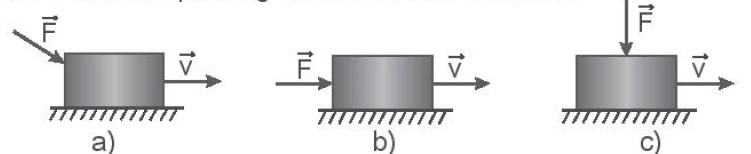
\includegraphics[width=0.4\linewidth]{../figs/VN10-2023-PH-TP024-P-5}
	\end{center}
	Độ lớn công do lực $F$ thực hiện xếp theo thứ tự tăng dần là
	\choice
	{(a), (b), (c)}
	{(a), (c), (b)}
	{(b), (a), (c)}
	{\True (c), (a), (b)}
	\loigiai{}
\end{ex}
% ===================================================================
\begin{ex}
	Một người kéo một thùng gỗ trượt trên sàn nhà bằng một sợi dây hợp với phương ngang một góc $\SI{60}{\degree}$, lực tác dụng lên dây là $\SI{200}{N}$. Khi thùng gỗ được kéo và trượt một đoạn $\SI{10}{m}$ thì công của lực kéo là	
	\choice
	{$\SI{200}{J}$}
	{\True $\SI{1000}{J}$}
	{$\SI{2000}{J}$}
	{$\SI{120000}{J}$}
	\loigiai{Công của lực kéo:
		$$A=Fs\cos \alpha = \SI{1000}{J}.$$}
\end{ex}	
% ===================================================================
\begin{ex}
	$\SI{1}{\watt}$ bằng
	\choice
	{$\SI{1}{\joule\cdot\second}$}
	{\True $\SI{1}{\joule/\second}$}
	{$\SI{10}{\joule\cdot\second}$}
	{$\SI{10}{\joule/\second}$}
	\loigiai{}
\end{ex}
% ===================================================================
\begin{ex}
	Một bóng đèn sợi đốt có công suất $\SI{100}{\watt}$ tiêu thụ năng lượng $\SI{1000}{\joule}$. Thời gian thắp sáng bóng đèn là
	\choice
	{$\SI{1}{\second}$}
	{\True $\SI{10}{\second}$}
	{$\SI{100}{\second}$}
	{$\SI{1000}{\second}$}
	\loigiai{}
\end{ex}
% ===================================================================
\begin{ex}
	Một động cơ điện cung cấp công suất $\SI{15}{kW}$ cho một cần cẩu nâng vật có khối lượng 1 tấn lên cao $\SI{15}{m}$. Thời gian tối thiểu để thực hiện công việc này bằng bao nhiêu? Lấy $g=\SI{10}{m/s^2}$.
	\choice
	{$\SI{12}{s}$}
	{\True $\SI{10}{s}$}
	{$\SI{14}{s}$}
	{$\SI{18}{s}$}
	\loigiai{Áp dụng công thức tính công suất:
		$$\calP = \dfrac{A}{t} \Rightarrow t = \dfrac{A}{\calP}  = \dfrac{mgs}{\calP} = \SI{10}{s}.$$}
\end{ex}
% ===================================================================
\begin{ex}
	Để nâng một tảng đá có trọng lượng $\SI{500}{\newton}$ lên như hình, một người sử dụng đòn bẩy bằng cách tác dụng một lực $\SI{180}{\newton}$ vào một đầu đòn bẩy làm cho đầu đòn bẩy dịch chuyển $\SI{70}{\centi\meter}$ còn tảng đá dịch chuyển $\SI{20}{\centi\meter}$. Hiệu suất của đòn bẩy là
	\begin{center}
		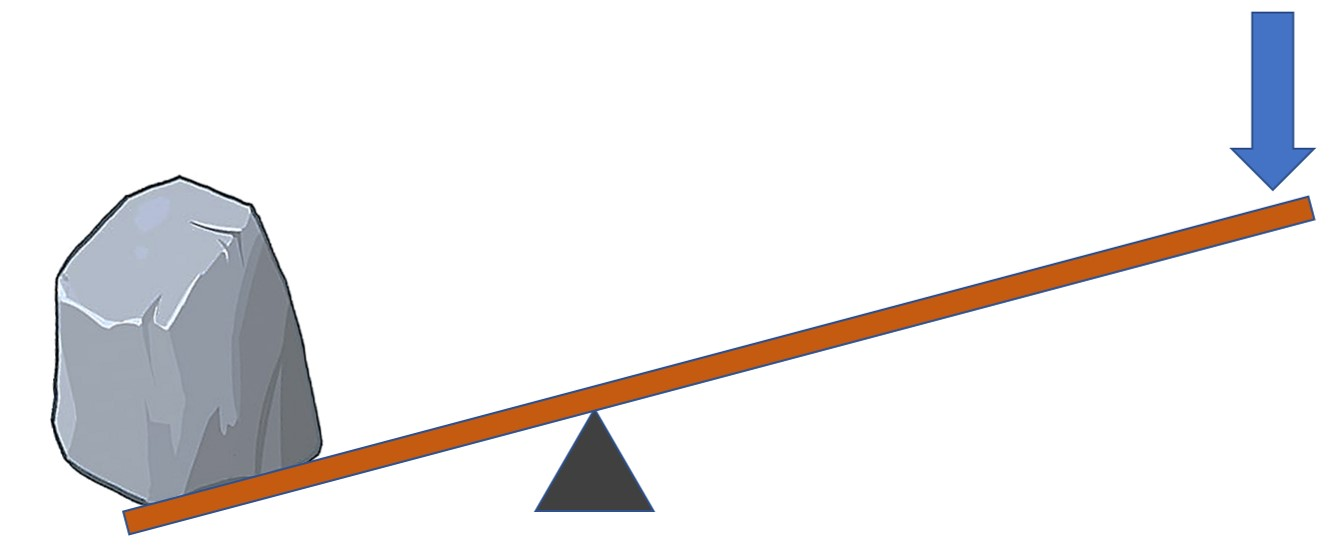
\includegraphics[width=0.4\linewidth]{../figs/VN10-2022-PH-TP023-P-12}
	\end{center}
	\choice
	{$\SI{126}{\percent}$}
	{$\SI{97.2}{\percent}$}
	{$\SI{36.0}{\percent}$}
	{\True $\SI{79.4}{\percent}$}
	\loigiai{}
\end{ex}

% ===================================================================
\begin{ex}
	Một máy bơm nước mỗi giây có thể bơm được 15 lít nước lên bể ở độ cao $\SI{10}{\meter}$. Hiệu suất của máy bơm là 0,7. Lấy $g=\SI{10}{\meter/\second^2}$. Biết khối lượng riêng của nước là  $D=\SI{E3}{\kilogram/\meter^3}$. Sau nửa giờ máy bơm đã thực hiện một công bằng	
	\choice
	{$\SI{1500}{\kilo\joule}$}
	{\True $\SI{3857}{\kilo\joule}$}
	{$\SI{1890}{\kilo\joule}$}
	{$\SI{7714}{\kilo\joule}$}
	\loigiai{Khối lượng nước được bơm lên sau nửa giờ:
		$$m=D\cdot V=\left(\SI{1000}{\kilogram/\meter^3}\right)\cdot\left(\SI{15E-3}{\meter^3}\right)\cdot\left(\SI{1800}{\second}\right)=\SI{27E3}{\kilogram}$$
		Công có ích máy bơm cần thực hiện để bơm lượng nước trên lên cao $\SI{10}{\meter}$:
		$$A_i=mgh=\SI{2700}{\kilo\joule}$$
		Công toàn phần máy bơm thực hiện:
		$$A_\text{tp}=\dfrac{A_i}{H}=\SI{3857}{\kilo\joule}.$$}
\end{ex}
\Closesolutionfile{ans}
\section{TRẮC NGHIỆM ĐÚNG/SAI}
\setcounter{ex}{0}
\Opensolutionfile{ans}[ans/D10-CONGVACONGSUAT-TF]
% ===================================================================
\begin{ex}
	Nhận định tính đúng/sai của các phát biểu sau khi nói về công của lực tác dụng lên vật.
	\choiceTF[t]
	{\True Vật rơi tự do thì trọng lực tác dụng lên vật sinh công dương}
	{Khi vật trượt lên mặt phẳng nghiêng thì lực ma sát giữa vật và mặt nghiêng sinh công dương}
	{Cần cẩu nâng đều khối vật liệu lên tòa nhà cao tầng thì trọng lực không thực hiện công}
	{Khi xe chuyển động chậm dần thì lực kéo của động cơ sinh công âm}
	\loigiai{}
\end{ex}
% ===================================================================
\begin{ex}
	Một cái thùng $\SI{50}{\kilogram}$ được đẩy lên $\SI{6.0}{\meter}$ theo mặt phẳng nghiêng góc $\SI{30}{\degree}$ với tốc độ  không đổi bởi một lực $\vec{F}$ không đổi như hình. Hệ số ma sát trượt giữa thùng và mặt nghiêng là $0,20$. Biết $\mathrm{AM}=\mathrm{MB}$.
	\begin{center}
		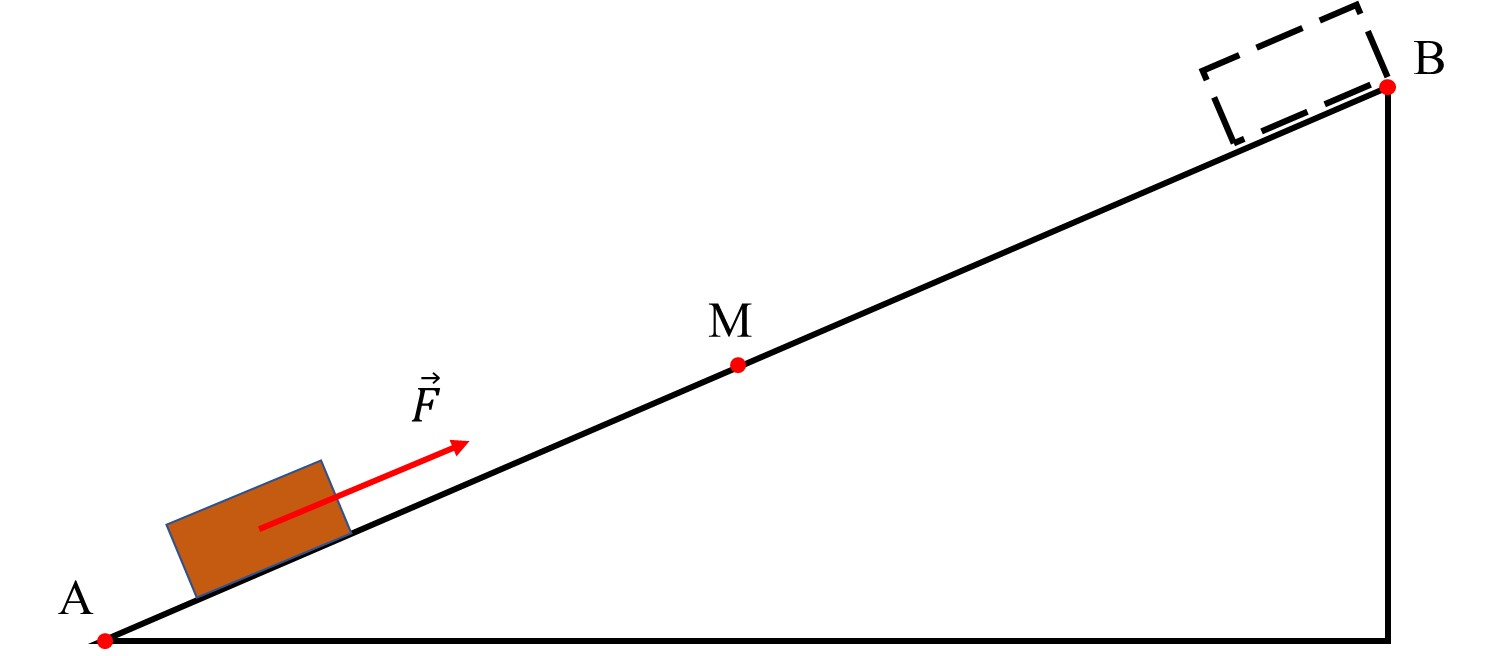
\includegraphics[scale=0.35]{../figs/VN10-2023-PH-TP024-P-8}
	\end{center}
	\choiceTF[t]
	{Công của trọng lực tác dụng lên thùng là công phát động}
	{Công của lực ma sát tác dụng lên thùng trên đoạn AM có giá trị lớn hơn trên đoạn AB}
	{Công của phản lực bằng công của trọng lực}
	{\True Độ lớn công của lực kéo bằng tổng độ lớn công của trọng lực và độ lớn công của lực ma sát}
	\loigiai{
	\begin{itemchoice}
		\itemch Sai. Trọng lực sinh công âm.
		\itemch Sai. $\mathrm{AM}=\mathrm{MB}$ nên công lực ma sát trên 2 đoạn là như nhau.
		\itemch Sai. Phản lực $\vec{N}$ vuông góc hướng chuyển động nên không sinh công.
		\itemch Đúng. Áp dụng định lý động năng, do vật chuyển động với tốc độ không đổi nên $\sum A=0\Rightarrow A_F=-A_{F_{\mathrm{ms}}}-A_P$. Lực kéo sinh công dương, lực ma sát và trọng lực sinh công âm nên  độ lớn công của lực kéo bằng tổng độ lớn công trọng lực và độ lớn công lực ma sát.
	\end{itemchoice}
	}
\end{ex}
% ===================================================================
\begin{ex}
	Một ô tô có khối lượng 1 tấn đang chuyển động trên đường. Giai đoạn đầu, ô tô chuyển động thẳng đều trên mặt đường nằm ngang với tốc độ $\SI{36}{\kilo\meter/\hour}$ với công suất trung bình của động cơ là \SI{5}{\kilo\watt}. Giai đoạn sau, ô tô tăng tốc chuyển động nhanh dần đều và sau khi đi thêm được $\SI{125}{\meter}$ thì đạt tốc độ $\SI{54}{\kilo\meter/\hour}$. Biết độ lớn lực ma sát không đổi trong suốt quá trình ô tô chuyển động.
	\choiceTF[t]
	{\True Giai đoạn đầu, lực ma sát của mặt đường tác dụng lên ô tô là $\SI{500}{\newton}$}
	{\True Gia tốc của ô tô trong giai đoạn chuyển động nhanh dần đều là $\SI{0.5}{\meter/\second^2}$}
	{\True Khi ô tô chuyển động nhanh dần đều thì lực kéo của động cơ bằng $\SI{1000}{\newton}$}
	{\True Giai đoạn sau, công suất trung bình của động cơ ô tô sau khi đi thêm $\SI{125}{\meter}$ là $\SI{12.5}{\kilo\watt}$}
	\loigiai{
	\begin{itemchoice}
		\itemch Đúng.\\ 
		Lực kéo của động cơ trong giai đoạn đầu:
		$F_k=\dfrac{\calP}{v_0}=\SI{500}{\newton}$.\\
		Vì ô tô chuyển động thẳng đều nên $F_{\mathrm{ms}}=F_k=\SI{500}{\newton}$.
		\itemch Đúng. $a=\dfrac{v^2-v^2_0}{2s}=\SI{0.5}{\meter/\second^2}$.
		\itemch Đúng. $F'_k=F_{\mathrm{ms}}+ma=\SI{1000}{\newton}$.
		\itemch Đúng. $\calP_{\mathrm{tb}}=F'_kv_{\mathrm{tb}}=F'_k\cdot\left(\dfrac{v+v_0}{2}\right)=\SI{12.5}{\kilo\watt}$.
	\end{itemchoice}
	}
\end{ex}
\section{TỰ LUẬN}
\setcounter{ex}{0}
\Opensolutionfile{ans}[ans/D10-CONGVACONGSUAT-TL]
% ======================================================================
\begin{ex}
	Mỗi tế bào cơ trong cơ thể người có thể coi như một động cơ siêu nhỏ, khi con người hoạt động, tế bào cơ sử dụng năng lượng hoá học để thực hiện công. Trong mỗi nhịp hoạt động, tế bào cơ có thể sinh một lực $\SI{1.5E-12}{\newton}$ để dịch chuyển $\SI{8}{\nano\meter}$. Tính công mà tế bào cơ sinh ra trong mỗi nhịp hoạt động.	
	\loigiai{$A=Fs\cos\SI{0}{\degree}=\SI{1.2E-20}{\joule}$}
\end{ex}
% ======================================================================
\begin{ex}
	Một hành khách kéo đều một vali đi trong nhà ga trên sân bay trên quãng đường dài $\SI{150}{m}$ với lực kéo có độ lớn $\SI{40}{N}$ theo hướng hợp với phương ngang một góc $\SI{60}{\degree}$. Hãy xác định công của lực kéo của người này.
	\loigiai{Công của lực kéo của người: $$A=Fs\cos \alpha = \SI{3000}{J}.$$}
\end{ex}
% ======================================================================
\begin{ex}
	\immini{Một kĩ sư xây dựng nặng $\SI{75}{\kilogram}$ trèo lên một chiếc thang dài $\SI{2.75}{\meter}$. Thang được dựa vào bức tường thẳng đứng và tạo một góc $\alpha=\SI{75}{\degree}$ với mặt phẳng ngang.
	\begin{enumerate}[label=\alph*)]
		\item Tính công của trọng lực tác dụng lên kĩ sư khi người này leo từ chân đến đỉnh thang.
		\item Đáp án của câu a có phụ thuộc vào tốc độ của người kĩ sư trong quá trình leo không?
		\end{enumerate}}
	{\vspace{-0.5cm}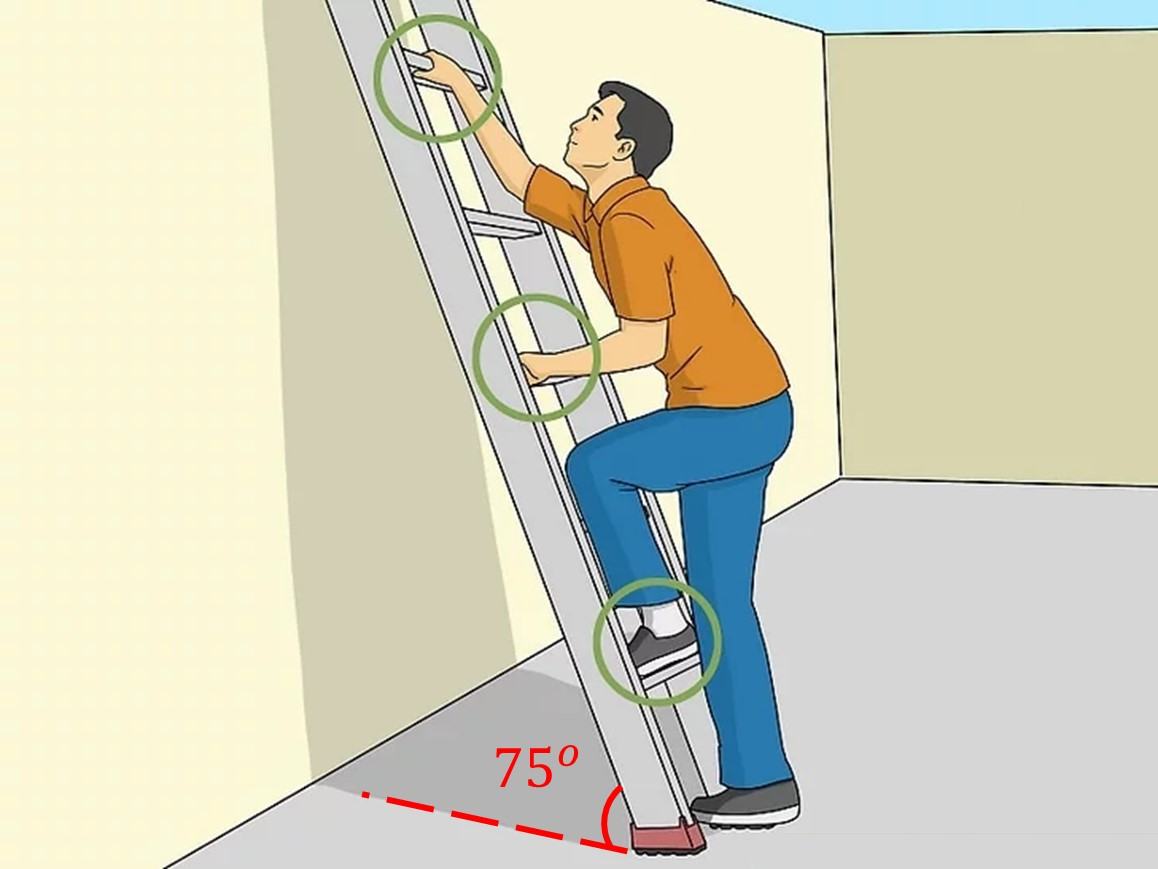
\includegraphics[scale=0.3]{../figs/VN10-2023-PH-TP024-P-3}}
	\loigiai{
		\begin{enumerate}[label=\alph*)]
			\item $$A_P=-mg\ell\sin\alpha\approx\SI{-1992.2}{\joule}.$$
			\item Không phụ thuộc vào tốc độ của người kĩ sư trong quá trình leo.
		\end{enumerate}
	}
\end{ex}
% ======================================================================
\begin{ex}
	\immini{Một người y tá đẩy bệnh nhân nặng $\SI{87}{\kilogram}$ trên chiếc xe băng ca nặng $\SI{18}{\kilogram}$ làm cho bệnh nhân và xe băng ca chuyển động thẳng trên mặt sàn nằm ngang với gia tốc không đổi là $\SI{0.55}{\meter/\second^2}$. Bỏ qua ma sát giữa bánh xe và mặt sàn.
	\begin{enumerate}[label=\alph*)]
		\item Tính công mà y tá đã thực hiện khi bệnh nhân và xe băng ca chuyển động được $\SI{1.9}{\meter}$.
		\item Sau quãng đường dài bao nhiêu thì y tá sẽ tiêu hao một công là $\SI{140}{\joule}$?
	\end{enumerate}
	}
{
\includegraphics[scale=1.4]{../figs/VN10-2023-PH-TP024-P-6}}
	\loigiai{
		\begin{enumerate}[label=\alph*)]
			\item $F=(m+m')a=\SI{57.75}{\newton}$\\
			$A=Fs\cos\SI{0}{\degree}\approx\SI{109.7}{\joule}$.
			\item $s'=\dfrac{A'}{F}=\SI{2.4}{\meter}$.
		\end{enumerate}
	}
\end{ex}
% ======================================================================
\begin{ex}
	Kỉ lục trong leo cầu thang được xác lập vào ngày 4/2/2003. Theo đó một vận động viên đã leo 86 tầng với 1576 bậc cầu thang trong 9 phút 33 giây. Mỗi bậc cầu thang cao $\SI{20}{\centi\meter}$ và vận động viên nặng $\SI{70}{\kilogram}$. Tính công suất trung bình của vận động viên này.
	\loigiai{
		Quãng đường đi: $s=1576\cdot0,2=\SI{315.2}{\meter}$.\\
		Công suất trung bình của vận động viên:
		$$\calP=\dfrac{A}{t}=\dfrac{mgs}{t}\approx\SI{377.4}{\watt}.$$
	}
\end{ex}
% ======================================================================
\begin{ex}
	Khi đưa một vật lên cao $\SI{2,5}{m}$ bằng mặt phẳng nghiêng, người ta phải thực hiện một công là $\SI{3600}{J}$. Biết hiệu suất của mặt phẳng nghiêng là $\SI{75}{\percent}$. Tính khối lượng của vật đó. Lấy $g = \SI{10}{m/s}^2$.	
	\loigiai{Ta có:
		$$H = \dfrac{A_\text{i}}{A_{\mathrm{tp}}} = \dfrac{mgh}{A_{\mathrm{tp}}}\Rightarrow m=\SI{10,8}{\kilogram}.$$
	}
\end{ex}
% ======================================================================
\begin{ex}
	Động cơ của máy bay Airbus A320 có công suất $\SI{384}{HP}$. Để cất cánh tốt nhất, máy bay cần đạt tốc độ $\SI{308}{\kilo\meter/\hour}$. Khi bay ở độ cao ổn định, tốc độ trung bình của máy bay là $\SI{1005}{\kilo\meter/\hour}$ và để tiết kiệm nhiên liệu thì tốc độ trung bình là $\SI{968}{\kilo\meter/\hour}$. Tính lực kéo máy bay trong từng trường hợp trên. Biết $\SI{1}{HP} \approx \SI{746}{\watt}$.
	\loigiai{
		Công suất động cơ $\calP=384\cdot746=\SI{286464}{\watt}$.\\
		Lực kéo của động cơ máy bay trong từng trường hợp:
		\begin{itemize}
			\item Ở tốc độ $\SI{308}{\kilo\meter/\hour}$ ($v_1\approx\SI{85.6}{\meter/\second}$): $F_1=\dfrac{\calP}{v_1}\approx\SI{3346.5}{\newton}$.
			\item Ở tốc độ $\SI{1005}{\kilo\meter/\hour}$ ($v_2\approx\SI{279.2}{\meter/\second}$): $F_2=\dfrac{\calP}{v_2}\approx\SI{1026}{\newton}$.
			\item Ở tốc độ $\SI{968}{\kilo\meter/\hour}$ ($v_3\approx\SI{268.9}{\meter/\second}$): $F_3=\dfrac{\calP}{v_3}\approx\SI{1065.3}{\newton}$.
		\end{itemize}
	}
\end{ex}
% ======================================================================
\begin{ex}
	Một ô tô có khối lượng $m=\SI{1.30E3}{\kilogram}$ di chuyển trên đoạn đường ABCD có dạng như hình bên dưới, trong đó BC là đoạn đường nằm ngang ở độ cao $h=\SI{50.0}{\meter}$ so với mặt phẳng ngang chứa AD. Biết rằng $\text{BC}=\SI{20}{\kilo\meter}$, gia tốc rơi tự do $g=\SI{9.80}{\meter/\second^2}$, độ dài các cung cong nối các đoạn đường thẳng với nhau rất nhỏ so với chiều dài của các đoạn thẳng đó, hãy tính công của trọng lực trên các đoạn đường AB, BC, CD.
	\begin{center}
		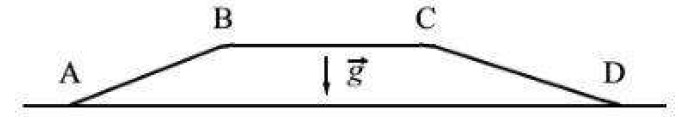
\includegraphics[scale=0.5]{../figs/VN10-2023-PH-TP024-P-7}
	\end{center}
	\loigiai{
		$A_{\mathrm{AB}}=-mgh=\SI{-637}{\kilo\joule}$; $A_{\mathrm{BC}}=0$; $A_{\mathrm{CD}}=mgh=\SI{637}{\kilo\joule}$.}
\end{ex}
% ======================================================================
\begin{ex}
	Một ô tô chuyển động đều với vận tốc $\SI{54}{km/h}$ có thể đi được đoạn đường dài bao nhiêu khi tiêu thụ hết 60 lít xăng? Biết động cơ của ô tô có công suất $\SI{45}{kW}$; hiệu suất $25\%$; $\SI{1}{kg}$ xăng đốt cháy hoàn toàn tỏa ra nhiệt lượng bằng $\xsi{46\cdot 10^6}{J/kg}$ và khối lượng riêng của xăng là $\SI{700}{kg/m^3}$.
	\loigiai{Đổi $\SI{54}{km/h} = \SI{15}{m/s}; \SI{45}{kW} = \SI{45000}{W}.$\\		
		Gọi $s$ là quãng đường đi được khi động cơ tiêu thụ hết 60 lít xăng.\\		
		Khối lượng 60 lít xăng:
		$$m = DV = \SI{42}{kg}.$$
		Công thực hiện của động cơ:
		$$A = \calP t = \calP \dfrac{s}{v}.$$
		Nhiệt lượng do 60 lít xăng khi bị đốt cháy hoàn toàn tỏa ra là 
		$$Q = qm.$$
		Ta có:
		$$H = \dfrac{A}{Q} \Rightarrow A = HQ  \Leftrightarrow P \dfrac{s}{v} = Hqm \Rightarrow s = \SI{161000}{m} = \SI{161}{km}.$$
		Vậy khi tiêu thụ hết 60 lít xăng, ô tô có thể đi được quãng đường là $\SI{161}{km}.$}
\end{ex}
% ======================================================================
\begin{ex}
	Một ô tô khối lượng 1 tấn đang hoạt động với công suất $\SI{5}{kW}$ và chuyển động thẳng đều với vận tốc $\SI{54}{km/h}$ thì lên dốc. Hỏi động cơ ô tô phải hoạt động với công suất bằng bao nhiêu để có thể lên dốc với tốc độ như cũ? Biết hệ số ma sát giữa bánh xe và mặt đường không đổi, dốc nghiêng góc $\SI{2,3}{^\circ}$ so với mặt đường nằm ngang và $g = \SI{10}{m/s}^2.$	
	\loigiai{Đổi 1 tấn $= \SI{1000}{kg}; \SI{5}{kW} = \SI{5000}{W}; \SI{54}{km/h} = \SI{15}{m/s}.$
		
		Khi xe ô tô chuyển động thẳng đều: 
		
		$$F'_\text{ms} = F'_\text{k} = \dfrac{\calP'}{v} = \xsi{\dfrac{1000}{3}}{\newton}.$$
		
		Hệ số ma sát là:
		
		$$\mu = \dfrac{F'_\text{ms}}{mg} = \dfrac{1}{30}.$$
		
		Khi ô tô chuyển động lên dốc, các lực tác dụng lên ô tô được biểu diễn 
		
		
		\begin{center}
			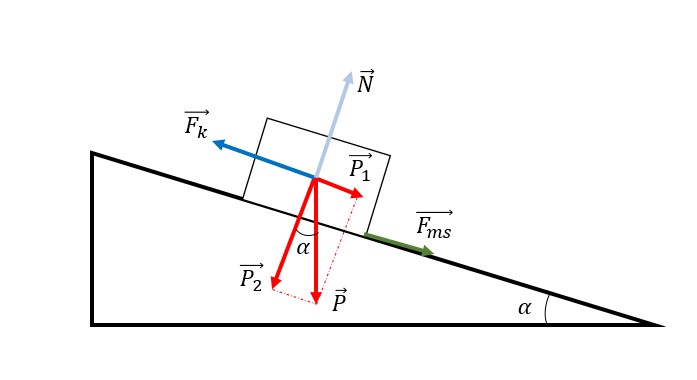
\includegraphics[scale=0.8]{../figs/VN10-2022-PH-TP027-1.jpg}
		\end{center}
		Khi lực kéo ô tô khi lên dốc có giá trị:
		$$F_\text{k} = F_\text{ms} + P_1 = \mu mg \cos \alpha + mg\sin \alpha = \SI{734,38}{N}.$$
		Để có thể lên dốc với tốc độ như cũ, ô tô phải hoạt động với công suất:
		$$\calP = F_\text{k} v = \SI{11015,7}{W}.$$}
\end{ex}
\Closesolutionfile{ans}
